\chapter{The Application Infrastructure}

The Fake news detetction system architecture is shown in\hyperref[fig:infrastructure]{Figure 3.1} it was inspired from balance transfer network [2]
 \begin{figure}[H]
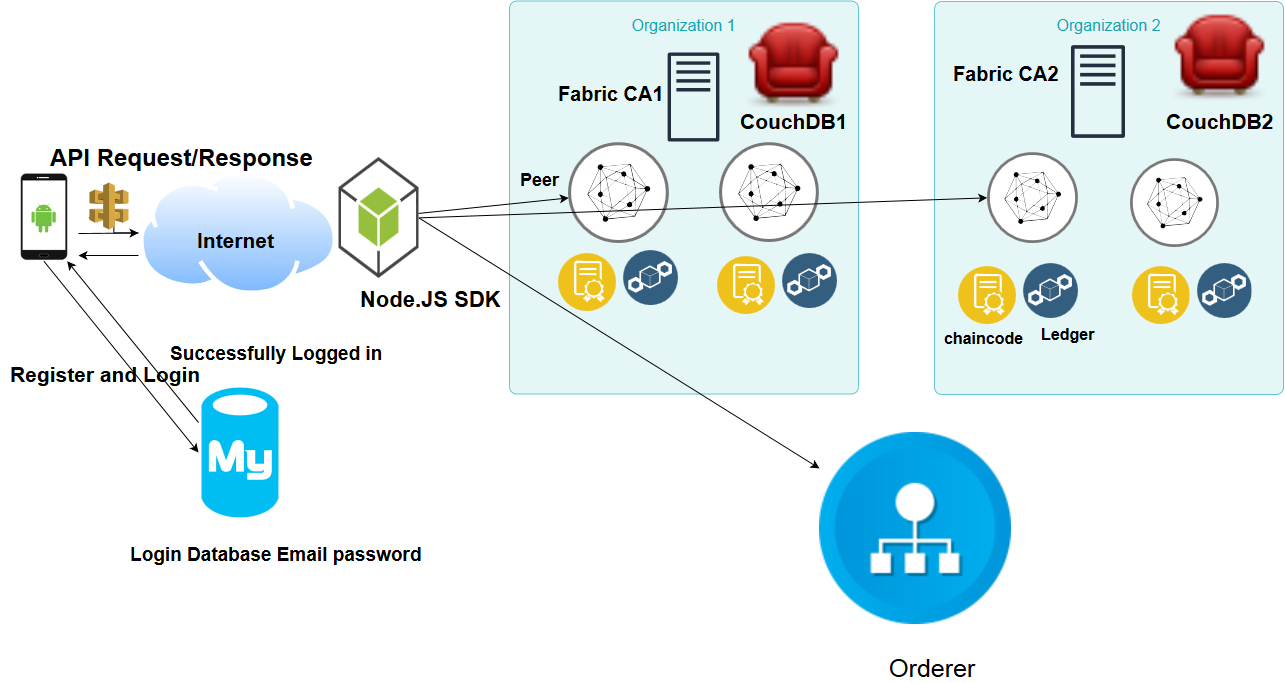
\includegraphics[width=15cm,height=12cm]{images/infrastructure.png}
\caption{The Application Infrastructure Overview}
\label{fig:infrastructure}
\end{figure}
\cleardoublepage

As shown the system comprises of Two Organizations Organization 1 and organization 2. with two peers in each organization. 
With a solo orderer node.  There are also two fabric CA Server one for each organization, a couchdb instance per organization for more efficient and rich queries. 
In addition, we are using node.js SDK  for interacting to the hyperledger fabric network and abstracting all the network infrastructure as a standard model thus the network could be scalable horizontally and vertically. All nodes are running on Docker containers for our testing purpose we implemented all the infrastructure on one Virtual Machine, However, in a production scenario every node should be an independent physical instance. \\ 

A layer of authentication using a traditional database was added, so that the users could sign up on our application using the traditional way we used email and password, however integrating a phone authentication with One time pad could be a trivial thing. 
Once the user successfully login he could send requests from android device using our application to the SDK. and the SDK will handle the interaction with hyperledger fabric network and the chaincode. 
 
The fabirc CA Server will be responsilbe for Registration of identities, Issuance of Enrollment Certificates for signing and identifying, Issuance of Transaction Certificates and Providing both anonymity and unlinkability when transacting on a Hyperledger Fabric blockchain. All these functionality are provided.
The network was an adoption of Balance transfer [2] A sample Node.js app to demonstrate fabric-client, fabric-ca-client and Node.js SDK APIs. 
the main idea of the network is to demontsrate a simple use case app using hyperledger fabric in order to transfer a balance from a user to another one and query the chaincode. we modified te network, added a couchdatabse instance and updating it with our chaincode. we modified the nodejs application to suit our application. 

Crypto material has been generated using the cryptogen tool from Hyperledger Fabric and mounted to all peers, the orderering node and CA containers. 
Beside An Orderer genesis block (genesis.block) and channel configuration transaction (mychannel.tx) has been pre generated using the configtxgen tool from Hyperledger Fabric and placed within the artifacts folder. 



\section{} 


 



 
  